\documentclass[10pt,journal,compsoc, onecolumn]{IEEEtran}

\pdfoutput=1 
\usepackage[varg]{txfonts}
\let\iint=\relax
\let\iiint=\relax
\let\iiiint=\relax
\let\idotsint=\relax

\let\subcaption\relax

\usepackage{amsmath}
\usepackage{amsfonts}
\usepackage{graphicx}
\usepackage{color}
\usepackage{ramkidefns}
%for displaying topic words
\usepackage{pgfplotstable}
\usepackage{longtable}
\usepackage{booktabs}
\usepackage{colortbl}

\newcommand{\ParNMF}{MPI-FAUN}

\begin{document}

\begin{center}
\huge
Supplement Material for MPI-FAUN
\end{center}

In this section, we present results from two of the real world datasets. 
The first example shows an image processing example of background separation and moving object detection in surveillance video data, and the second example shows topic modeling output on the \emph{stack exchange} text dataset. The details of these datasets are presented in Section 6.1.1. 
While the literature covers more detail about fine tuning NMF and different NMF variants for higher quality results on these two tasks  \cite{ZT2011,B2014,AGHKT2014,KJJCH2015}, our main focus is to show how quickly we can produce a baseline NMF output and its real world interpretation. 

\section{Moving Object Detection of Surveillance Video Data}

As explained in the Section 6.1.1, we processed 12 minutes video that is captured from a 
busy junction in Georgia Tech to separate the background and moving objects from this video. 
In Figure \ref{fig:videoresults}, we present some sample frames to compare the input image with the separated background and moving objects.
The background are the results of the low rank approximation 
$\hat{\AA}=\WW\HH$ output yielded from our \ParNMF\ algorithm and the moving objects are given by $\AA-\hat{\AA}$. 
We can clearly see the static background is captured in the second column and the moving objects (e.g., cars) are visible in the third column. 
The moving object matrix has been color-adjusted to make the cars more obvious, which has also magnified the noise.
%There are sufficient literature that utilizes the background $\hat{\AA}$ and produces a high  quality moving objects from the input image $\AA$, which is not the focus of this paper. 

\section{Topic Modeling of Stack Exchange Data}

We downloaded the latest Stack Overflow  dump from its archive on 28-Jul-2016. The details of 
the preprocessing and the sparse matrix generation are explained in Section 6.1.1. We ran 
our \ParNMF\ algorithm on this dataset, which has nearly 12 million questions from the Stack Overflow site (under Stack Exchange) to produce 50 topics. 
The matrix $\WW$ can be interpreted as {\em vocabulary-topic} distribution and the 
$\HH$ as {\em topic-document} distribution.  We took the top 5 words for each of the 50 topics and 
present them in Table \ref{tab:stackexchangetopics}. Typically a good topic generation satisfies 
properties such as (a) finding discriminative rather than common words -- capturing words that can provide 
some information; (b) finding different topics -- the similarity between different topics should be low; 
(c) coherence - all the words that belong to one topic should be coherent.  There are some topic quality 
metrics \cite{NLGB2010} that capture the usefulness of topic generation algorithm.  We can  see
 NMF generated generally high-quality and coherent topics. 
 Also, each of the topics are from different domains such as 
 databases, C/C++ programming, Java programming, and web technologies like PHP and HTML. 

%\pgfplotstableset{
%begin table=\begin{longtable},
%end table=\end{longtable},
%}

%\begin{table}
%\footnotesize
%\pgfplotstabletypeset[
%	col sep=comma,
%	every head row/.style={before row=\toprule,after row=\midrule},
%        every last row/.style={after row=\bottomrule},
%	columns={word1,word2,word3,word4,word5,word1,word2,word3,word4,word5},
%	display columns/0/.style={column type/.add={|}{}, select equal part entry of={0}{2}, string type},
%	display columns/1/.style={select equal part entry of={0}{2}, string type},
%	display columns/2/.style={select equal part entry of={0}{2}, string type},
%	display columns/3/.style={select equal part entry of={0}{2}, string type},
%	display columns/4/.style={column type/.add={}{||}, select equal part entry of={0}{2}, string type},
%	display columns/5/.style={column type/.add={>{\columncolor[gray]{.8}}}{},select equal part entry of={1}{2}, string type},
%	display columns/6/.style={column type/.add={>{\columncolor[gray]{.8}}}{},select equal part entry of={1}{2}, string type},
%	display columns/7/.style={column type/.add={>{\columncolor[gray]{.8}}}{},select equal part entry of={1}{2}, string type},
%	display columns/8/.style={column type/.add={>{\columncolor[gray]{.8}}}{},select equal part entry of={1}{2}, string type},
%	display columns/9/.style={column type/.add={>{\columncolor[gray]{.8}}}{},column type/.add={}{|}, select equal part entry of={1}{2}, string type},
%	%every even column/.style={column type/.add={>{\columncolor[gray]{.8}}}{}}
%	outfile=stackxchangetopics.tex
%]{data/topkwords.csv}
%\normalsize
%\caption{Top 5 words of 50 topics from {\em Stack Exchange} data set. \grey{Maybe make left 5 columns white and right 5 gray?  It's hard to see that there are two columns to connect the 5 related words.}}
%\label{tab:stackexchangetopics}
%\end{table}
%

\newcommand{\wdth}{1.65in}
\newcommand{\hght}{1.0725in}
\begin{figure*}[th!]
\centering
\begin{tabular}{ccc}
Input Frame($\AA$) & Background ($\WW\HH$) & Moving Object $\AA-\WW\HH$ \\
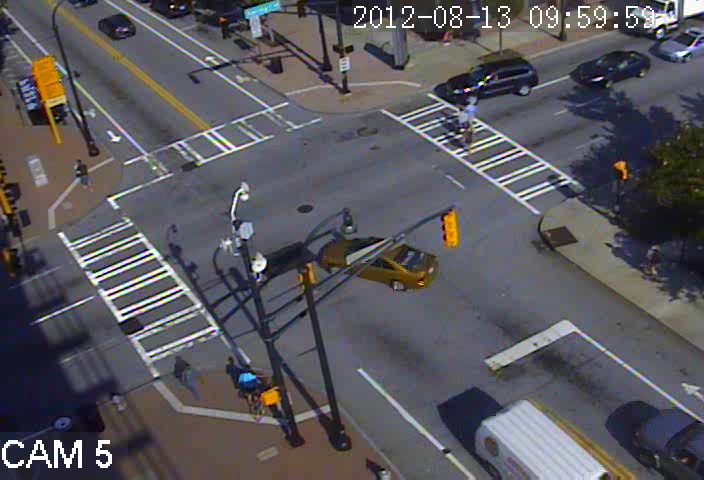
\includegraphics[height=\hght,width=\wdth]{fig/input1.png} &  
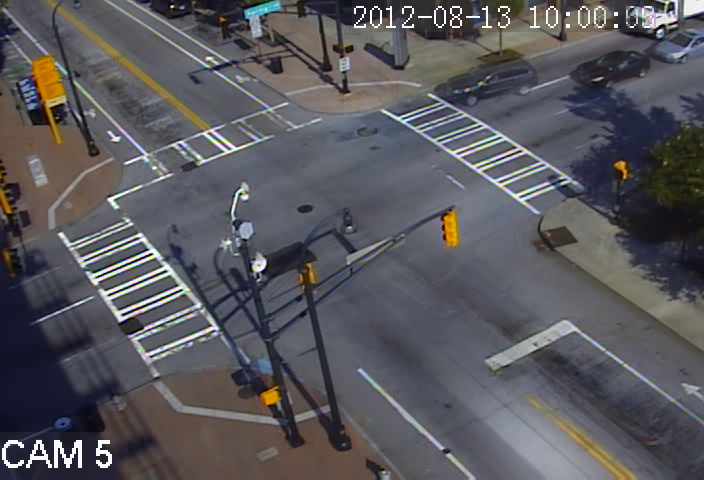
\includegraphics[height=\hght,width=\wdth]{fig/lr1.png}&
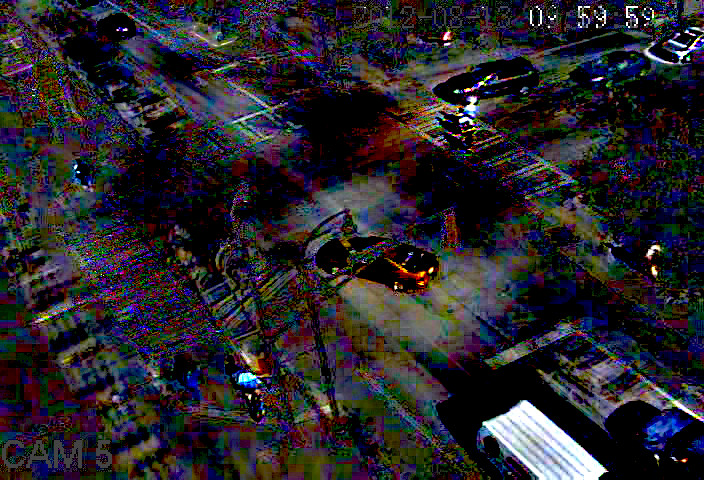
\includegraphics[height=\hght,width=\wdth]{fig/err1-edit.png} \\
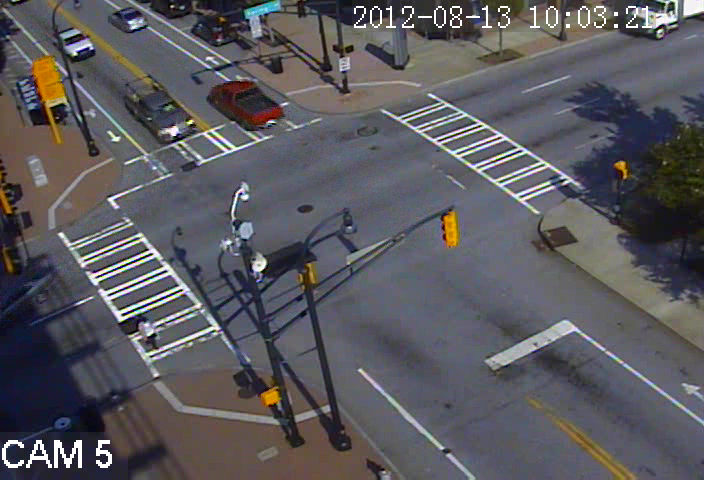
\includegraphics[height=\hght,width=\wdth]{fig/input4000.png} &  
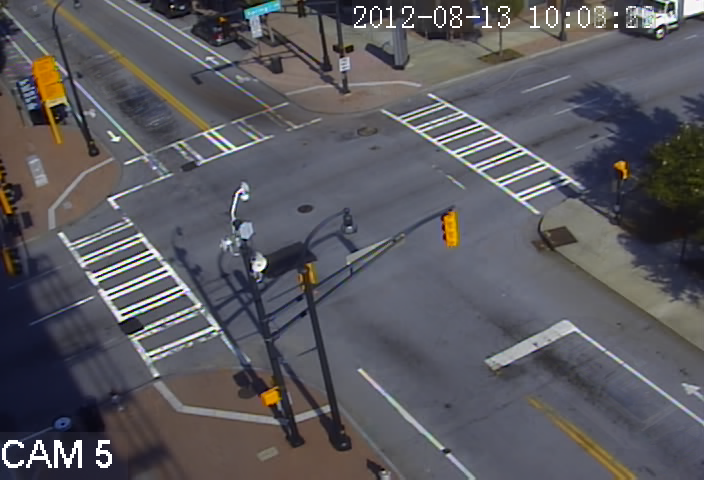
\includegraphics[height=\hght,width=\wdth]{fig/lr4000.png}&
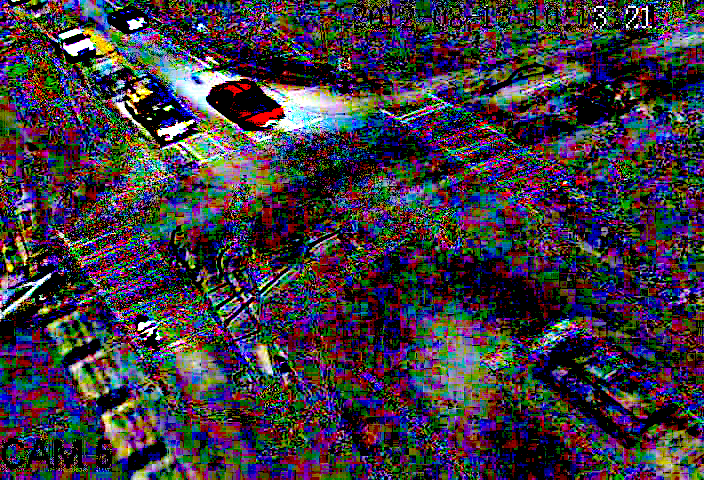
\includegraphics[height=\hght,width=\wdth]{fig/err4000-edit.png} \\
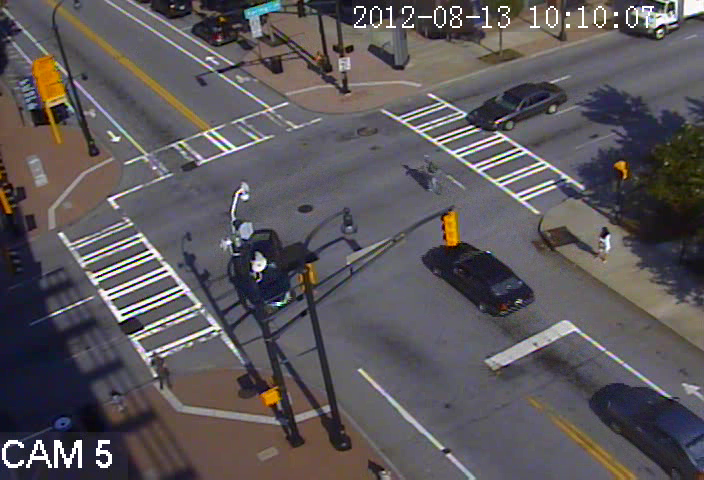
\includegraphics[height=\hght,width=\wdth]{fig/input12000.png} &  
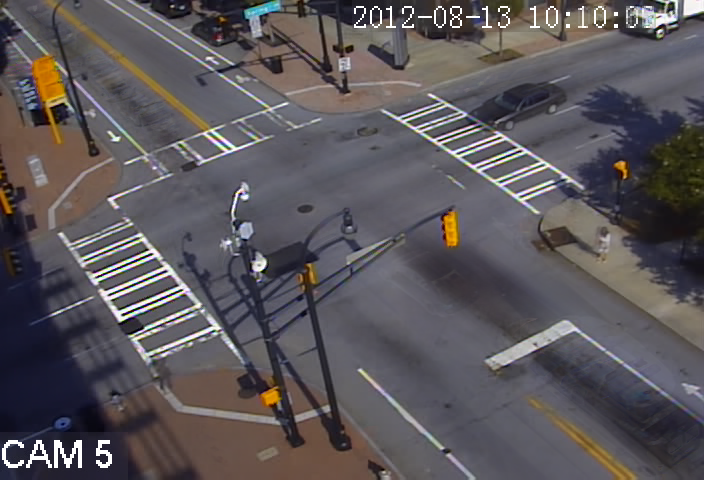
\includegraphics[height=\hght,width=\wdth]{fig/lr12000.png}&
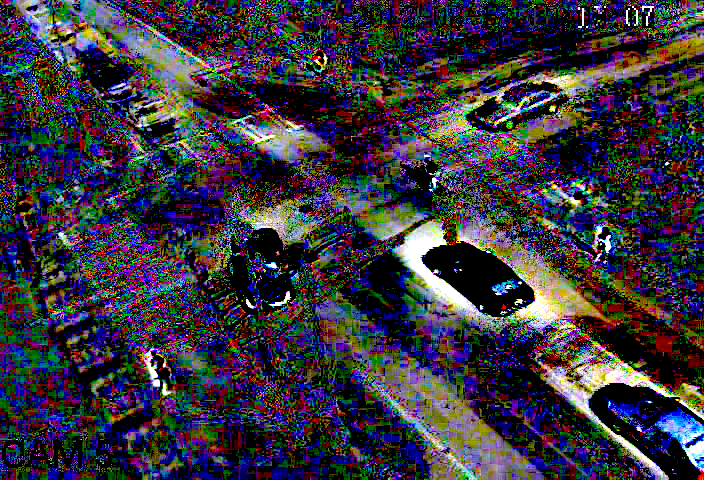
\includegraphics[height=\hght,width=\wdth]{fig/err12000-edit.png} \\
\end{tabular}
\caption{Moving object detection for video data using NMF.  Each row of images corresponds to a particular frame in the video.  The left column is the original frame, the middle column is the reconstructed frame from the low-rank approximation (which captures the background), and the right column is the difference (which captures the moving objects) with color adjustment.}
\label{fig:videoresults}
\end{figure*}

\begin{table*}[th!]
\begin{center}
\footnotesize
\begin {tabular}{|ccccc||>{\columncolor [gray]{.8}}c>{\columncolor [gray]{.8}}c>{\columncolor [gray]{.8}}c>{\columncolor [gray]{.8}}c>{\columncolor [gray]{.8}}c|}%
\toprule 
\multicolumn{5}{|c||}{Top Keywords from Topics 1-25} & \multicolumn{5}{|>{\columncolor [gray]{0.8}}c|}{Top Keywords from Topics 26-50} \\ 
word1&word2&word3&word4&word5&word1&word2&word3&word4&word5\\\midrule %
refer&undefin&const&key&compil&echo&type=text&php&form&result\\%
text&field&box&word&static&test&perform&fail&unit&result\\%
imag&src&descript&alt=ent&size&tabl&key&queri&databas&insert\\%
button&click&event&form&add&user&email&usernam&login&log\\%
creat&bean&add&databas&except&data&json&store&read&databas\\%
string&static&final&catch&url&page&load&content&url&link\\%
width&height&color&left&display&privat&static&final&import&float\\%
app&applic&servic&thread&work&row&column&date&cell&valu\\%
ipsum&lorem&dolor&sit&amet&line&import&command&print&recent\\%
node&list&root&err&element&var&map&marker&match&url\\%
0x00&0xff&byte&0x01&0xc0&server&connect&client&messag&request\\%
file&directori&read&open&upload&number&byte&size&print&input\\%
function&call&event&work&variabl&object&properti&json&instanc&list\\%
int&char&const&static&doubl&array&element&valu&key&index\\%
public&overrid&virtual&static&extend&main&thread&program&frame&cout\\%
return&param&result&def&boolean&type&field&properti&argument&resolv\\%
info&thread&start&map&servic&select&item&queri&join&list\\%
error&syntax&found&symbol&fail&sourc&target&except&java&fail\\%
set&properti&virtual&default&updat&instal&version&packag&err&default\\%
case&break&switch&default&cout&code&work&problem&chang&write\\%
method&call&except&static&todo&void&overrid&protect&catch&extend\\%
href&nofollow&src&link&work&true&requir&boolean&option&valid\\%
end&def&dim&begin&properti&find&project&import&warn&referenc\\%
debug&request&filter&match&found&view&control&item&overrid&posit\\%
fals&boolean&fix&bool&autoincr&null&default&key&int(11&primari\\\bottomrule %
\end {tabular}%

\normalsize
\end{center}
\caption{Top 5 words of 50 topics from {\em Stack Exchange} data set.}
%\grey{Maybe make left 5 columns white and right 5 gray?  It's hard to see that there are two columns to connect the 5 related words.}
\label{tab:stackexchangetopics}
\end{table*}

\bibliographystyle{IEEEtran}
\bibliography{paper}
\end{document}